\documentclass[12pt]{article}
\usepackage{graphicx} % Required for inserting images
\usepackage{geometry}
\geometry{a4paper, margin=2.5cm}
\usepackage[T1]{fontenc}
\usepackage{palatino}
\usepackage{amsmath, amssymb}
\usepackage{array}
\usepackage{titling}
\usepackage{subcaption}

\setlength{\droptitle}{-5em}
\preauthor{\begin{center}\large\vspace{0.5em}}
\postauthor{\end{center}\vspace{-0.5em}}

\title{{\scshape  Part IIB Revision Notes} \\ 
    \vspace{0.5em}
    \textbf{4F12: Computer Vision}}
\author{Qianshuo (Harry) Ye}
\date{April 2026}

\usepackage{parskip}
\begin{document}
\maketitle

\section{Feature Detection and Matching}
\textbf{Image structure:}
\begin{itemize}
    \item \textit{Featureless region:} smooth variation of intensities.
    \item \textit{Edge:} intensity discontinuity in one direction.
    \item \textit{Corner:} intensity discontinuity in two directions.
    \item \textit{Blob:} circular region of uniform intensity.
\end{itemize}

Central motivation for feature extraction: to reduce the amount of data to be processed.

Desirable properties of features:
\begin{itemize}
    \item Preserve the useful information in an image.
    \item Discard redundant information.
    \item Should be as generic as possible.
\end{itemize}

\textbf{1D edge detection:} The general procedure is
\begin{enumerate}
    \item Convolve the signal $I(x)$ with a Gaussian kernel $g_\sigma(x) = \frac{1}{\sigma\sqrt{2\pi}} \exp\left(-\frac{x^2}{2\sigma^2}\right)$.
    \item Compute the derivative $s'(x) = \frac{d}{dx} [I(x) * g_\sigma(x)]$.
    \item Find maxima and minima of $s'(x)$.
    \item Use thresholding to mark edges.
\end{enumerate}
To save computation, directly find zero crossings of $s''(x)$, obtained by convolving the signal with the \textit{Laplacian} of a Gaussian
$$
s''(x) = g_\sigma''(x) * I(x)
$$
The parameter $\sigma$ controls the scale of edge detection: larger $\sigma$ detects coarser edges.

Filtering effects:
\begin{itemize}
    \item Convolution with the Gaussian is \textit{low-pass} filtering: $g_\sigma(x) \leftrightarrow g_{\sigma'}(\omega), \sigma' = \frac{1}{\sigma}$.
    \item Convolution with the Laplacian is \textit{band-pass} filtering: $g_\sigma''(x) \leftrightarrow g_{\sigma'}''(\omega) = -\omega^2 g_{\sigma'}(\omega)$.
\end{itemize}

\textbf{2D edge detection:} The general procedure is similar to the 1D case, but the image is smoothed with a 2D Gaussian kernel
$$
G_\sigma(x, y) = \frac{1}{2\pi\sigma^2} \exp\left(-\frac{x^2 + y^2}{2\sigma^2}\right)
$$
\textit{Canny detector}: The gradient of the smoothed image $\nabla S$ is used to perform non-maximum suppresion: place edge elements (edgels) where $|\nabla S|$ is greater than local values of $|\nabla S|$ along the direction of $\pm \nabla S$. 
The edgels are thresholded -- only those with $|\nabla S|$ above a certain value are kept.

\textit{Marr-Hildreth operator}: Find the zero crossings of $\nabla^2 G_\sigma * I$, where $\nabla^2 G_\sigma$ is the Laplacian of the $G_\sigma$.

In practice, the convolution are performed as truncated summations (typically the discarded samples are $< 1/1000$ of the peak value, yielding a kernel of size $N = 2n+1$ where $n > 3.7 \sigma - 1$):
$$
S(x,y) = G_\sigma(x,y) * I(x,y) = \sum_{u=-n}^{n} \sum_{v=-n}^{n} G_\sigma(u,v) I(x-u, y-v)
$$
The 2D convolution can be decomposed into two 1D convolutions
$$
S(x,y) = g_\sigma(x) * [g_\sigma(y) * I(x,y)] = \sum_{u = -n}^{n} \sum_{v = -n}^{n} g_\sigma(u) g_\sigma(v) I(x-u, y-v)
$$
The computational saving is $\frac{(2n+1)^2}{2(2n+1)} = \frac{2n+1}{2}$.

Implementations:
\begin{itemize}
    \item Differentiation $\frac{\partial S}{\partial x}$: discrete convolution with the kernel $[1/2, 0, -1/2]$, using the approximation $\frac{\partial S}{\partial x} \approx \frac{S(x+1,y) - S(x-1,y)}{2}$.
    \item 1D Laplacian $\nabla^2S(x)$: discrete convolution with the kernel $[1, -2, 1]$, using the approximation $\nabla^2 S = \frac{\partial^2}{\partial x^2} I(x) \approx S(x+1) + S(x-1) - 2S(x)$.
    \item 2D Laplacian $\nabla^2S(x,y)$: discrete convolution with the kernel $\begin{bmatrix}
        0 & 1 & 0 \\
        1 & -4 & 1 \\
        0 & 1 & 0
    \end{bmatrix}$, using the approximation $\nabla^2 S = (\frac{\partial^2}{\partial x^2} + \frac{\partial^2}{\partial y^2})I(x,y) \approx S(x+1,y) + S(x-1,y) + S(x,y+1) + S(x,y-1) - 4S(x,y)$.
\end{itemize}

Limitations of edges as keypoints:
\begin{itemize}
    \item Edges only allow localisation in one dimension.
    \item Edges cannot be used to determine the scale of a feature.
\end{itemize}

\textbf{Corner detection:} One way is to compute the normalised cross-correlation between an image patch $P$ and other portions of the image $I$:
$$
c(x,y) = \frac{\sum_{u=-n}^{n} \sum_{v=-n}^{n} I(x+u, y+v) P(u,v)}{\sqrt{\sum_{u=-n}^{n} \sum_{v=-n}^{n} I(x+u, y+v)^2 \sum_{u=-n}^{n} \sum_{v=-n}^{n} P(u,v)^2}}
$$
A patch with a well-defined peak in its correlation function is a corner.

A more efficient method is to use the intensity difference:
\begin{enumerate}
    \item Calculate change in intensity in direction $\mathbf{n}$:
    \begin{align*}
        S_n &= \nabla S(x,y) \cdot \hat{\mathbf{n}} = [S_x \quad S_y]^\top \cdot \hat{\mathbf{n}} \approx S(\mathbf{x}+\hat{\mathbf{n}}) - S(\mathbf{x})\\
        S_n^2 &= \frac{\mathbf{n}^\top \begin{bmatrix}
            S_x^2 & S_x S_y \\
            S_x S_y & S_y^2
        \end{bmatrix} \mathbf{n}}{\mathbf{n}^\top \mathbf{n}}
    \end{align*}
    \item Smooth $S_n^2$ with a Gaussian kernel:
    $$
    C_n(x,y) = G_\sigma * S_n^2 = \frac{\mathbf{n}^\top \overbrace{\begin{bmatrix}
            \langle S_x^2 \rangle & \langle S_x S_y \rangle \\
            \langle S_x S_y \rangle & \langle S_y^2 \rangle
        \end{bmatrix}}^{A} \mathbf{n}}{\mathbf{n}^\top \mathbf{n}}
    $$
    where $\langle \cdot \rangle$ denotes the smoothed value.
    \item According to eigenvector theory, $\lambda_1 \leq C_n(x,y) \leq \lambda_2$. $\lambda_1$ and $\lambda_2$ are eigenvalues of $A$. $\lambda_2$ is the maximum smoothed change in intensity and $\lambda_1$ is the minimum.
    A corner is detected if $\lambda_1$ and $\lambda_2$ are \textit{both large and distinct}.
\end{enumerate}

The \textit{Harris-Stephens corner detector} computes the 
\begin{itemize}
    \item determinant $\text{det}(A) = \lambda_1 \lambda_2$ 
    \item and the trace $\text{Tr}(A) = \lambda_1 + \lambda_2$
\end{itemize}
A corner is detected when $\lambda_1 \lambda_2 - \kappa (\lambda_1 + \lambda_2)^2$ is greater than some threshold.

\textbf{Blob detection:}
\begin{itemize}
    \item Convolution with the Laplacian of Gaussian (LoG) kernel produce a strong response with an extrema at the center of a blob when the scale of the kernel $\sigma$ matches the size of the blob. 
    \item The radius of the matched blob is $\sqrt{2} \sigma$ (where zero-crossing occurs).
\end{itemize}

\textbf{Image pyramids:} A sequence of images smootheed with Gaussians of different scales. The scale satisfies $\sigma_{i} = 2^{i/s} \sigma_0$ so it doubles every $s$ levels. 

To construct an image pyramid:
\begin{itemize}
    \item The image is smoothed incrementally by convolution $G(\sigma_{i+1}) = G(\sigma_i) * G(\sigma_{k_i})$.
    \item The scale for the incremental blur is $\sigma_{k_i} = \sqrt{\sigma_{i+1}^2 - \sigma_i^2} = \sigma_i \sqrt{2^{2/s} - 1}$ (only need to be computed once). A total of $s$ incremental blurs are needed in an octave.
    \item After $s$ levels, $\sigma_s = 2 \sigma_0$, subsample the image to 1/4 of the original size by skipping every other row and column.
    \item Repeat the process to construct the next octave of the pyramid, reusing the incremental blurs $\sigma_{k_i}$.
\end{itemize}

\textbf{Difference of Gaussian (DoG):} A blob detector that approximates the LoG:
\begin{align*}
G(x,y, k\sigma) - G(x,y,\sigma) &\approx (k-1) \sigma^2 \nabla^2 G(x,y,\sigma) \\
G(x,y, \sigma_{i+1}) - G(x,y, \sigma_i) &\approx (2^{1/s}-1) \sigma_i^2 \nabla^2 G(x,y,\sigma_i)
\end{align*}
\textbf{Keypoint detection:} 
\begin{itemize}
    \item Blob centeres are found by subtracting neighbouring images of in the image pyramid and search for local extrema.
    \item The local extrema is located by comparing with 26 neighbouring pixels in the current, upper and lower levels.
    \item Normalise for scale of the keypoint by sampling neighbouring pixels in the appropriate image of the image pyramid.
\end{itemize}
\textbf{Keypoint orientation:} 
\begin{itemize}
    \item Build a histogram (36 bins covering 360 degrees) of edge orientations weighted by their gradient magnitudes in a $16 \times 16$ neighbourhood.
    \item The gradients needs to be smoothed by a 2D Gaussian of size $1.5 \sigma$.
    \item The highest peak in the histogram is the dominant orientation.
    \item Normalise for orientation by sampling neighbouring pixels after computing a dominant orientation.
\end{itemize}

\begin{center}
    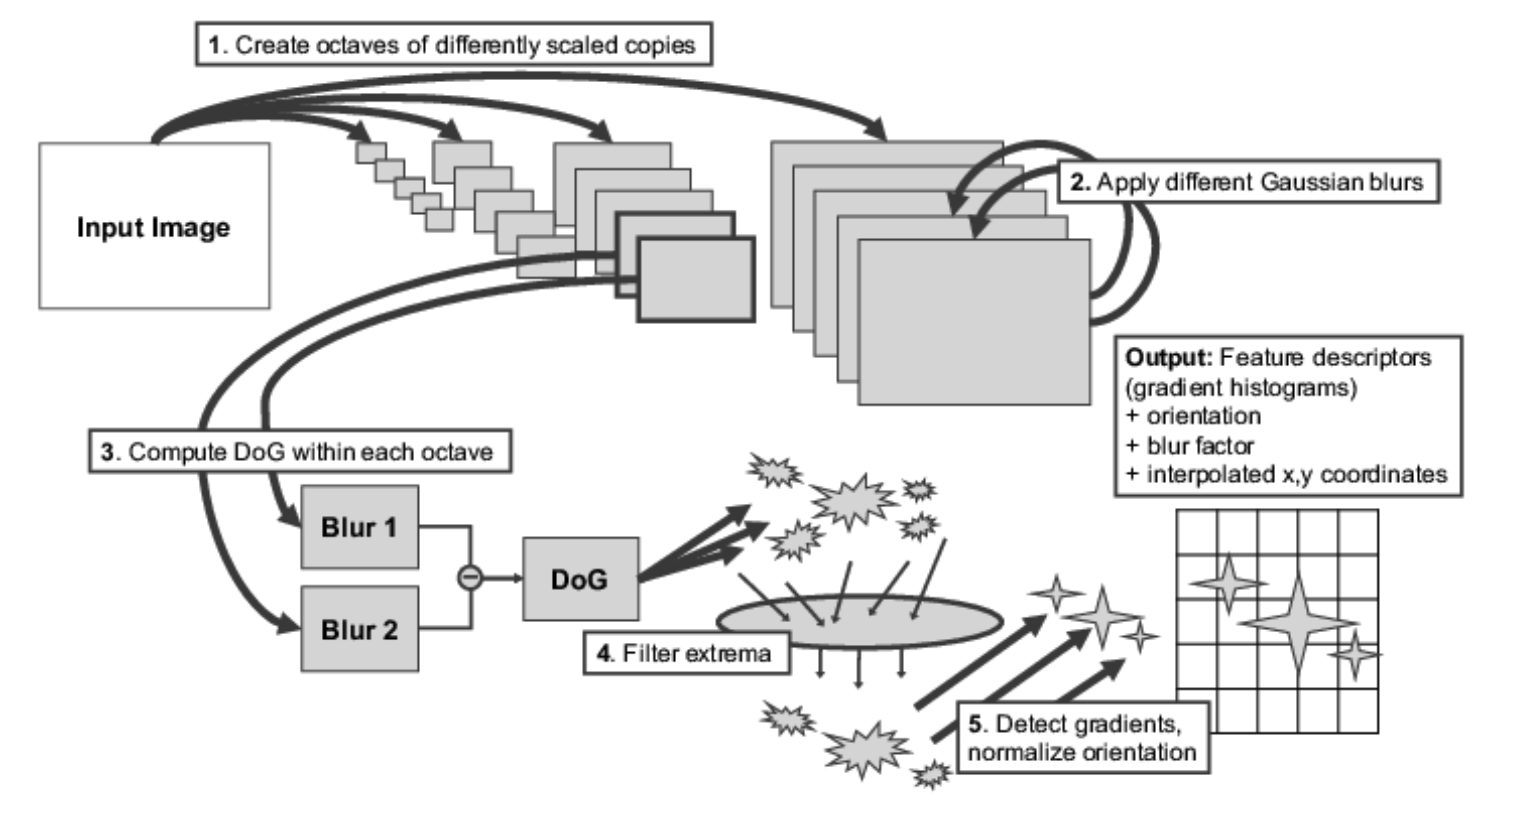
\includegraphics[width=0.8\textwidth]{figures/4F12/keypoint_detection.png}
\end{center}

\textbf{Normalised intensities descriptor:} Patches of intensities can be matched by the cross-correlation:
$$
CC(P_1, P_2) = \sum_i^N P_1[i] P_2[i]
$$
The patch can be normalised to make the matching invariant to changes in brightness and contrast:
\begin{align*}
    \mu &= \frac{1}{N}\sum_{x,y} I(x,y), \quad Z(x,y) = I(x,y) - \mu \\
    \sigma^2 &= \frac{1}{N} \sum_{x,y} Z(x,y)^2, \quad P(x,y) = \frac{Z(x,y)}{\sigma}
\end{align*}

\textbf{Scale-Invariant Feature Transform (SIFT) descriptor:} encodes 2D shapes by looking at gradients in a local neighbourhood, invariant to: position, scale, orientation and lighting.

Implementation:
\begin{enumerate}
    \item Split $N \times N$ patch into $c$ cells, calculate gradient at every pixel
    \item For each cell, build a histogram of gradient directions ($d$ directions) weighted by their magnitude and a Gaussian window with a $\sigma$ of $0.5$ times the feature scale (to avoid occlusion).
    \item Normalise the descriptor to make it invariant to changes in gradient magnitude (lighting).
    \item Threshold the maximum value of the descriptor to 0.2 to reduce the effect of strong lights, then renormalise.
\end{enumerate}
Typically, $N=16$, $c=16$ and $d=8$, so the SIFT descriptor is a 128-dimensional vector.

Limitations: The SIFT descriptor perform poorly at occluded object boundaries and large changes in viewpoint.

Invariances of SIFT:
\begin{itemize}
    \item \textit{Translation invariance:} the descriptor is computed at the location of a keypoint.
    \item \textit{Scale invariance:} the desciptor is computed from 16 $\times$ 16 pixels at the characteristic scale of a keypoint.
    \item \textit{Rotation invariance:} gradient orientations are stored relative to the dominnant orientation.
    \item \textit{Partial occlusion invariance:} the gradients are weighted by a Gaussian to reduce influence of gradients far from the centre.
    \item \textit{Local positional invariance:} historgrams are computed over cells of 4 $\times$ 4 pixels, so gradients can shift up to 4 pixels while still contributing to the same histogram.
    \item \textit{Local rotational invariance:} gradient orientations are aggregated in histograms with relativelt coarse bins.
    \item \textit{Affine illumination invariance:} the SIFT descriptor is normalised to unit length.
    \item \textit{Non-linear illumination invariance:} the values in the descriptor are thresholded.
\end{itemize}

A match can be measured by the Euclidean distance between two SIFT descriptors (linear search):
$$
E(\boldsymbol{x}, \boldsymbol{y}) = \sqrt{\sum_d (x_d - y_d)^2}
$$
The \textit{nearest neighbour search} can be performed viaa k-d tree. Accept a match if the distance to the nearest neighbour is less than 0.7 times the distance to the second nearest neighbour (ratio test):
$$
\frac{E(\boldsymbol{x}_m, \boldsymbol{x}_1)}{E(\boldsymbol{x}_m, \boldsymbol{x}_2)} < 0.7
$$

\textbf{Texture:} Orderly and repetitive patterns of regular sub-elements called \textit{textons}. Textures can be described by their response to a collection of filters.

\section{Projection}
\textbf{Orthographic projection:} Project the scene onto an image plan using parallel rays. The projection is given by
$$
\mathbf{x} = \mathbf{X} - (\mathbf{X} \cdot \mathbf{k}) \mathbf{k} = (\mathbf{k} \times \mathbf{X}) \times \mathbf{k}
$$

\textbf{Perspective projection:} Project the scene onto an image plane using rays that converge at a single point (the camera center). The projection is given by
$$
\mathbf{x} = \frac{f}{Z_c}\begin{bmatrix}
    X_c \\
    Y_c
\end{bmatrix}
$$
where $f$ is the focal length and $Z_c$ is along the optical axis.

Assumptions: pin-hole camera, central planar projection, no non-linear distortion.

\begin{center}
    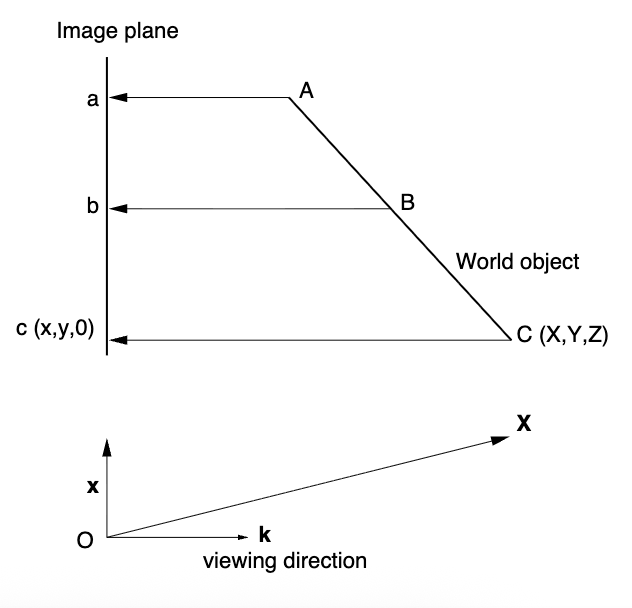
\includegraphics[width=0.4\textwidth]{figures/4F12/orthographic.png}
    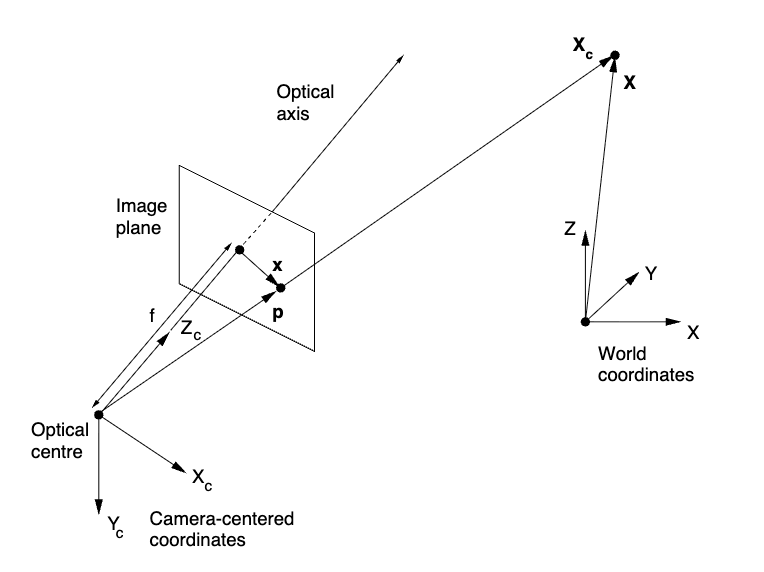
\includegraphics[width=0.5\textwidth]{figures/4F12/perspective.png}
\end{center}

\textbf{Vanishing points:} Points where parallel lines in the world meet in the image. Parallel plane meet in a line in the image called the \textit{horizon line}. Any set of parallel lines on the planes will have a vanishing point on the horizon line.
Vertical lines have a vanishing point at infinity.

\textbf{Full camera model:} A full camera describes the mapping fro world to pixel coordinates, consisting of 3 transformations:
\begin{enumerate}
    \item Rigid body motion between camera and the scene -- from world coordinates to camera coordinates:
    $$
    \mathbf{X}_c = \mathrm{R} \mathbf{X} + \mathbf{T} \text{ (rotation and translation)}
    $$
    \item Perspective projection -- mapping 3D points to 2D image plane:
    $$
    x = \frac{fX_c}{Z_c}, \quad y = \frac{fY_c}{Z_c}
    $$
    \item CCD imaging -- mapping the image plane to pixel coordinates:
    $$
    u = u_0 + k_u x, \quad v = v_0 + k_v y
    $$
\end{enumerate}

\textbf{Homogeneous coordinates:} represent each point in the image plane by a 3D vector and each point in the world by a 4D vector:
$$
\tilde{\mathbf{X}}_c = \begin{bmatrix}
    \lambda X_c \\
    \lambda Y_c \\
    \lambda Z_c \\
    \lambda
\end{bmatrix}
\quad
\tilde{\mathbf{x}} = \begin{bmatrix}
    s x \\
    s y \\
    s
\end{bmatrix}
$$
The homogeneous equations are
$$
a_1 X_c + a_2 Y_c + a_3 Z_c + a_4 = 0
\quad
b_1 x + b_2 y + b_3 = 0
$$
Points are at infinity when $\lambda = 0$ or $s = 0$. $\tilde{\mathbf{X}} = \mathbf{0}$ is undefined.

Perspective projection can be expressed as:
$$
\tilde{\mathbf{x}}= \begin{bmatrix}
    s x \\
    s y \\
    s
\end{bmatrix} = 
\begin{bmatrix}
    f & 0 & 0 & 0 \\
    0 & f & 0 & 0 \\
    0 & 0 & 1 & 0
\end{bmatrix}
\begin{bmatrix}
    \lambda X_c \\
    \lambda Y_c \\
    \lambda Z_c \\
    \lambda
\end{bmatrix} = \mathrm{P}_p \tilde{\mathbf{X}}_c
$$

\textbf{Camera projection matrix}: The full camera model can be expressed as
\begin{align*}
\mathbf{\tilde{w}} &= \mathrm{P}_{ps} \tilde{\mathbf{X}} = \mathrm{P}_c \mathrm{P}_p \mathrm{P}_r \tilde{\mathbf{X}} \\
\text{where } \mathrm{P}_r &= \begin{bmatrix}
    \mathrm{R} & \mathbf{T} \\
    \mathbf{0}^\top & 1
\end{bmatrix} \quad
\mathrm{P}_p = \begin{bmatrix}
    f & 0 & 0 & 0 \\
    0 & f & 0 & 0 \\
    0 & 0 & 1 & 0
\end{bmatrix}
\quad
\mathrm{P}_c = \begin{bmatrix}
    k_u & 0 & u_0 \\
    0 & k_v & v_0 \\
    0 & 0 & 1
\end{bmatrix}
\end{align*}
$\mathrm{P}_c \mathrm{P}_p$ accounts for the \textit{intrinsic} camera parameters, while $\mathrm{P}_r$ accounts for the \textit{extrinsic} parameters.

The projection matrix can be decomposed into a \textit{camera calibration matrix} $\mathbf{K}$ and a rigid body motion $[R|\mathbf{T}]$: $\mathrm{P}_{ps} = \mathbf{K} [R|\mathbf{T}]$, where
$$\mathbf{K} = \begin{bmatrix}
    f k_u & 0 & u_0 \\
    0 & f k_v & v_0 \\
    0 & 0 & 1
\end{bmatrix}$$
The ratio $f k_v / f k_u$ is the \textit{aspect ratio}.

\textbf{Projective camera:} A more general camera model, described by a $3 \times 4$ matrix $\mathrm{P}$.

When viewing a plane, the projection is a $homography$ that can be described by a $3 \times 3$ matrix.
When viewing a line, the projection can be described by a $3 \times 2$ matrix.

The degree of freedom of the matrices are $n - 1$ as the scale factor is arbitrary.

\textbf{Planar transformation:} Mapping between two planes.

Affine planar transformation is suitable when all points on the plane lie at approximately the same depth from the camera compared to the viewing distance. 

For affine planar transformation, there are 6 DoF: rotations (1), scaling (1), shear (2), translation (2).
General planar transformation have 2 extra DoFs that specify fanning.

\begin{center}
    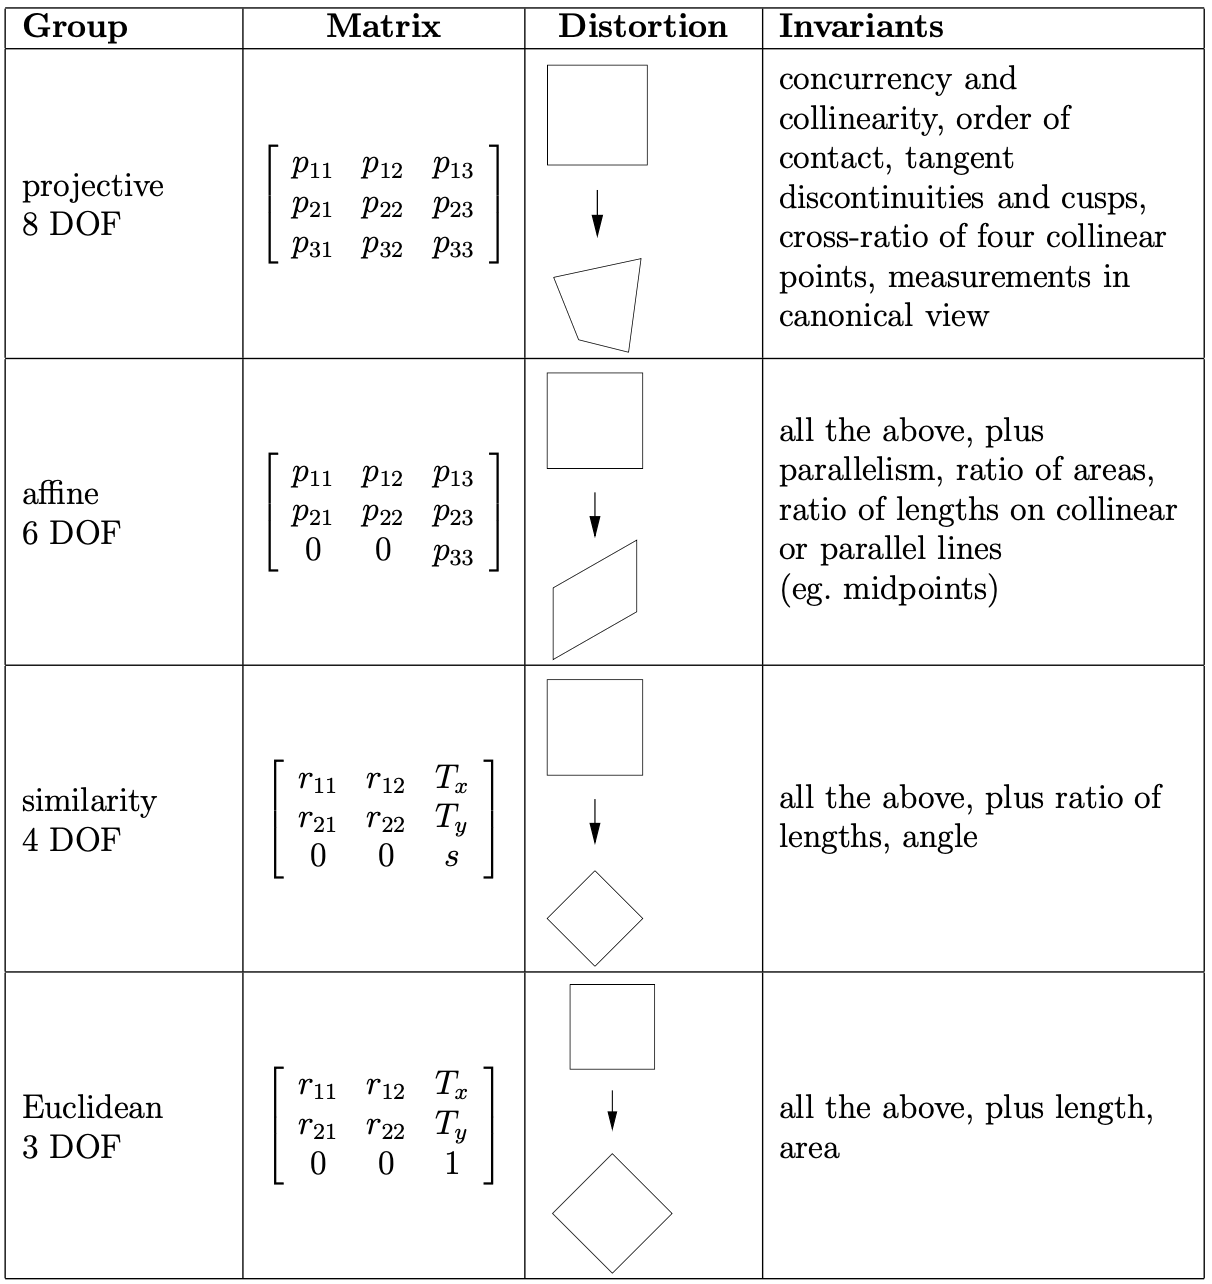
\includegraphics[width=0.6\textwidth]{figures/4F12/planar_transformation.png}
\end{center}

A circle in the world can be described by the equation:
$$
\mathbf{\tilde{X}}^\top \mathrm{C} \tilde{\mathbf{X}} = 0
$$
Under perspective projection $\mathbf{\tilde{w}} = \mathrm{H} \mathbf{\tilde{X}}$, the circle is projected to an ellipse described by
$$
\mathbf{\tilde{w}}^\top \mathrm{C}' \mathbf{\tilde{w}} = 0 \quad \text{where} \quad \mathrm{C}' = \mathrm{H}^{-\top} \mathrm{C} \mathrm{H}^{-1}
$$

\textbf{Camera calibration:} The process of determining the projection matrix $\mathrm{P}$. 

Desirable properties of the 3D objects for calibration inlcude:
\begin{itemize}
    \item Span large field of view.
    \item Easy to localise accurately and match.
    \item Must not be coplanar or collinear.
\end{itemize}

Each point $(u_i, v_i)$ gives 2 equations, so at least 6 points are needed to calibrate the camera.

The equations can be solve by linear least squares:
\begin{itemize}
    \item Arrange the equations in the form of $\mathrm{A} \mathbf{p} = 0$. 
    \item $\mathbf{p}$ is the eigenvector corresponding to the smallest eigenvalue of the $A^\top A$, which minimises the Rayleigh quotient
    $$
    \lambda_1 \leq \frac{\mathbf{p}^\top \mathrm{A}^\top \mathrm{A} \mathbf{p}}{\mathbf{p}^\top \mathbf{p}} \leq \lambda_{12}
    $$
\end{itemize}

The solution can be refined by non-linear minimisation of errors (between measured and projected points):
$$
\min_{\mathrm{P}} \sum_i ((u_i - \hat{u}_i)^2 + (v_i - \hat{v}_i)^2)
$$
Once $\mathrm{P}$ is known, decompose the $3\times 3$ submatrix into $\mathbf{K}$ and $\mathrm{R}$ using QR decomposition, and $\mathbf{T}$ can be found by $\mathbf{T} = \mathbf{K}^{-1} \begin{bmatrix}
    p_{14} & p_{24} & p_{34}
\end{bmatrix}^\top$.

To calibrate the camera for viewing a plane, at least 4 points are needed; for viewing a line, at least 3 points are needed.

\textbf{Recovery of world position:} The position of the point on the line can be uniquely determined by $u$. The position of the point on a plane can be determined by $u$ and $v$. The 3D position of the point cannot be uniquely determined by $u$ and $v$ alone -- it can only define a ray in space.

\textbf{Image mosaicing:} Any two images of a general scene with the same camera centre (rotation only) are related by
$$
\mathbf{\tilde{w}}' = \mathbf{K} \mathrm{R} \mathbf{K}^{-1} \mathbf{\tilde{w}}
$$
Tha camera is rotated around the optical centre an a sequence of image is aquired, with each image overlapping its predecessor to some extend. A minimum of 4 correspondences can be used to estimate the homography $\mathrm{H} = \mathbf{K} \mathrm{R} \mathbf{K}^{-1}$ between images and dispaly them in the same plane.

With many data ouliers, the homography can be estimated by RANSAC (RANdom SAmple Consensus):
\begin{enumerate}
    \item Match features points between two views
    \item Select minimal subset of matches (4 for homography)
    \item Compute the homography $\mathrm{H}$ from the subset
    \item Compute projected position and count the number of inliers (distance < threshold)
    \item Repeat steps 2-4 to maximise the number of inliers
\end{enumerate}

\textbf{Weak perspective projection:} When the range of depths of objects in the scene is small compared to their distance from the camera, the projection can be approximated as a parallel projection, with a weak perspective projection matrix
$$\mathrm{P}_{pll} = \begin{bmatrix}
    f & 0 & 0 & 0 \\
    0 & f & 0 & 0 \\
    0 & 0 & 0 & Z_c^{av}
\end{bmatrix}$$

\textbf{Affine camera:} The affine camera generalises the weak perspective projection.
$$
\mathrm{P}_{aff} = \begin{bmatrix}
    p_{11} & p_{12} & p_{13} & p_{14} \\
    p_{21} & p_{22} & p_{23} & p_{24} \\
    0 & 0 & 0 & 1
\end{bmatrix}
$$
The 3D affine camera can be calibrated by at least 4 points, a 2D one can be calibrated by at least 3 points, and a 1D one can be calibrated by at least 2 points.

Advantages of affine cameras:
\begin{itemize}
    \item Can be calibrated by fewer points.
    \item Calibration process is better conditioned (less sensitive to noise).
\end{itemize}

\textbf{Cross-ratio:} For 4 collinear points $a$, $b$, $c$ and $d$, the cross-ratio is defined as
$$
\frac{(X_d - X_a)(X_c - X_b)}{(X_c - X_a)(X_d - X_b)}
$$
\begin{center}
    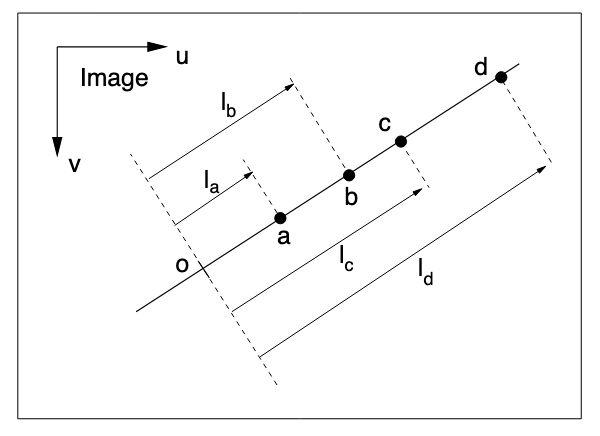
\includegraphics[width=0.3\textwidth]{figures/4F12/cross-ratio.png}
    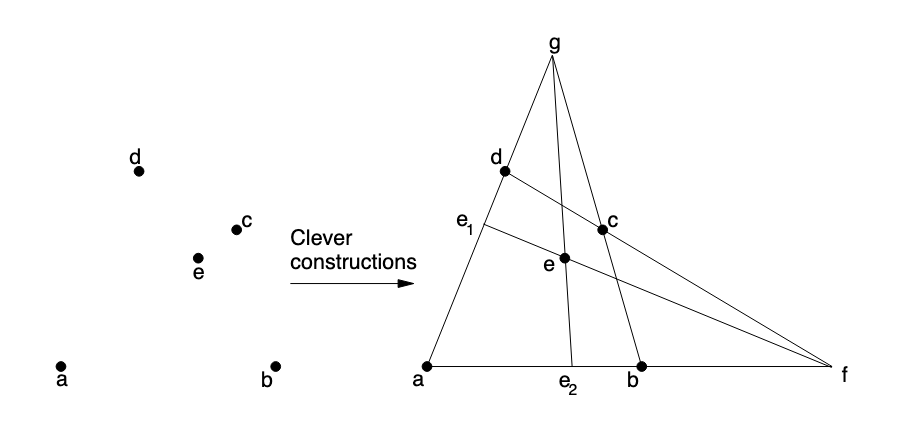
\includegraphics[width=0.5\textwidth]{figures/4F12/five_points_invariant.png}
\end{center}
The cross-ratio is invariant under projection. 5 points in a plane can be used to construct two cross-ratios.

\section{Stereo Vision}
\textbf{Rays:} A ray is define by the point it pierces the image plane
$$
\mathbf{p} = \begin{bmatrix}
    x \\
    y \\
    f
\end{bmatrix} \quad \text{and} \quad
\tilde{\mathbf{w}} = \mathbf{K}\mathbf{p}
$$

\begin{center}
    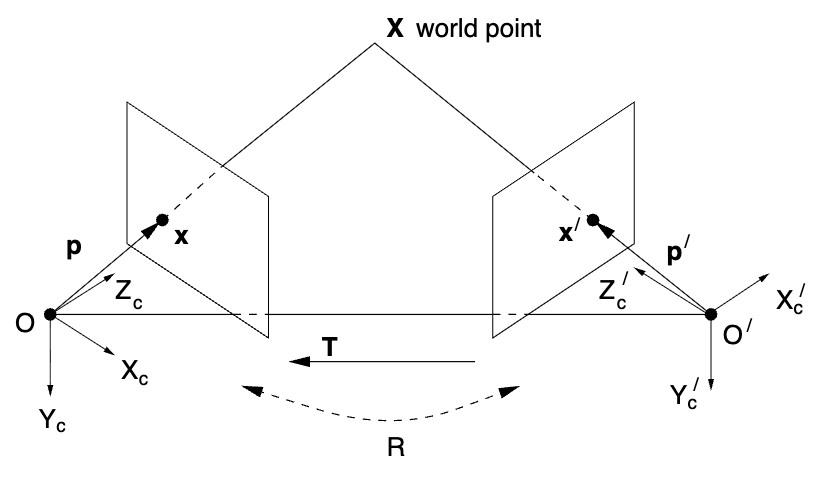
\includegraphics[width=0.45\textwidth]{figures/4F12/rays.png}
    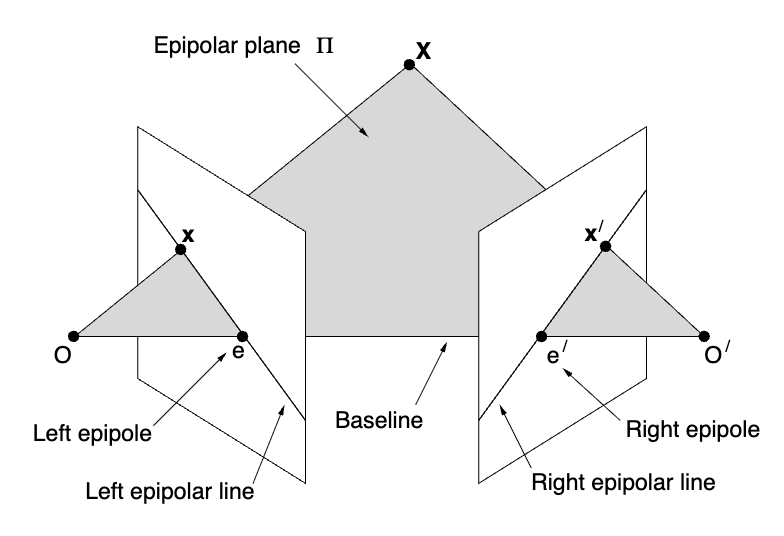
\includegraphics[width=0.45\textwidth]{figures/4F12/epipolar_geometry.png}
\end{center}

\textbf{Epipolar constraint:} Correspondences must lie on the epipolar lines.
\begin{itemize}
    \item An \textit{epipolar line} is the image of the ray from the other camera's optical centre to the point $\mathbf{X}$. 
    \item An \textit{epipole} is the image of the other camera's optical centre. All epipolar lines pass through the epipole.
\end{itemize}

The epipolar constraint can be expressed as 
$$
\mathbf{p}'^\top \mathrm{E} \mathbf{p} = 0
$$
where $\mathrm{E}$ is the \textit{essential matrix}, which can be decomposed into a vector product matrix of the translation $\textrm{T}_\times$ and a rotation matrix $\mathrm{R}$ between the two cameras:
$$
\mathrm{E} = \textrm{T}_\times \mathrm{R} \quad \text{where} \quad
\textrm{T}_\times = \begin{bmatrix}
    0 & -T_z & T_y \\
    T_z & 0 & -T_x \\
    -T_y & T_x & 0
\end{bmatrix}
$$
The epipoles follow $\mathrm{E} \mathbf{p}_e = \mathbf{0}$ and $\mathrm{E}^\top \mathbf{p}_e' = \mathbf{0}$. Hence, the $\mathrm{E}$ have a non-zero null space and is non-invertible.

Derivation:
\begin{align*}
    \mathrm{X_c'} &= \mathrm{R} \mathrm{X_c} + \mathbf{T} \\
    \mathbf{T} \times \mathrm{X_c'} &= \mathbf{T} \times (\mathrm{R} \mathrm{X_c} + \mathbf{T}) = \mathbf{T} \times \mathrm{R} \mathrm{X_c} \\
    \mathrm{X_c} \cdot (\mathbf{T} \times \mathrm{X_c'}) &= \mathrm{X_c}^\top (\mathbf{T} \times \mathrm{R} \mathrm{X_c}) = 0 \\
    \mathrm{X_c'}^\top [\textrm{T}_\times \mathrm{R}] \mathrm{X_c} &= \lambda^2 \mathbf{p}'^\top \mathrm{E} \mathbf{p} = 0
\end{align*}
The left epipole in the right camera's coordinates is 
$$
\lambda \mathbf{T} = \mathrm{R} \mathbf{p}_e \quad \rightarrow \quad \lambda \mathbf{T} \times \mathbf{T} = \mathbf{T} \times \mathrm{R} \mathbf{p}_e = \mathrm{E} \mathbf{p}_e = \mathbf{0}
$$

For parallel cameras, the epipolar lines are parallel and the epipoles are at infinity.

\textbf{Fundamental matrix:} Since $\mathbf{p} = \mathbf{K}^{-1}\tilde{\mathbf{w}}$, the fundamental matrix $\mathrm{F}$ can be defined as
$$
\mathrm{F} = \mathbf{K}'^{-\top} \mathrm{E} \mathbf{K}^{-1} \quad \text{such that} \quad \tilde{\mathbf{w}}'^\top \mathrm{F} \tilde{\mathbf{w}} = 0
$$
The epipolar lines follow $\tilde{\mathbf{l}}' = \mathrm{F} \tilde{\mathbf{w}}$ and $\tilde{\mathbf{l}} = \mathrm{F}^\top \tilde{\mathbf{w}}'$, and the epipoles follow $\mathrm{F} \tilde{\mathbf{w}}_e = \mathbf{0}$ and $\mathrm{F}^\top \tilde{\mathbf{w}}_e' = \mathbf{0}$.

Estimation:
Since the overall scale is arbitrary and the determinant is zero, the fundamental matrix has 7 degrees of freedom. The fundamental matrix can be estimated by at least 8 correspondences. 

If the correspondences are noisy, the estimate will not have zero determinant -- can be solved by setting the smallest singular value to zero.

\textbf{Constraints on the correspondences:}
\begin{enumerate}
    \item \textit{Epipolar constraint:} Each point feature identified in one image must lie on a corresponding epipolar line in the other image.
    \item \textit{Uniqueness:} For opaque objects, each point in the left image has at most one match in the right image.
    \item \textit{Ordering:} For an opaque object, the points are ordered identically in two images.
    \item \textit{Figural continuity:} If the distinguished points lie on contours, they can sometimes be matched by the continuity of the contours.
    \item \textit{Disparity gradient:} If surfaces are smooth, the disparities (differences between locations of corresponding points) must be locally smooth.
\end{enumerate}

\textbf{Finding correspondences:}
\begin{enumerate}
    \item Unguided matching: Use normalised cross-correalation to obtain a small number of seed matches.
    \item Compute epipolar geometry: Use seed matches and robust regression to estimate the fundamental matrix $\mathrm{F}$.
    \item Guided matching: Restrict the search for matches to a narrow band around epipolar lines.
\end{enumerate}

\textbf{Recovering metric structure:} The singular value decomposition of the essential matrix gives
$$
\mathrm{E} = \mathrm{U} \Lambda \mathrm{V}^\top = \mathrm{T}_\times \mathrm{R} \quad \text{where} \quad
\mathrm{T}_\times = \mathrm{U} \begin{bmatrix}
    0 & 1 & 0 \\
    -1 & 0 & 0 \\
    0 & 0 & 0
\end{bmatrix} \mathrm{U}^\top \quad \text{and} \quad
\mathrm{R} = \mathrm{U} \begin{bmatrix}
    0 & -1 & 0 \\
    1 & 0 & 0 \\
    0 & 0 & 1
\end{bmatrix} \mathrm{V}^\top
$$
which can be used to find the projection matrices:
$$
\mathrm{P} =\mathbf{K}\begin{bmatrix}
    \mathrm{I} & \mathbf{0}
\end{bmatrix} \quad \text{and} \quad
\mathrm{P}' = \mathbf{K}' \begin{bmatrix}
    \mathrm{R} & \mathbf{T}
\end{bmatrix}
$$
The projection matrices can be used to provide an initial estimate of the 3D coordinates of the matched points by triangulation. The reconstruction can be iteratively refined by minimising the \textit{reprojection error} through updating the 3D coordinates and the projection matrices -- the \textit{bundle adjustment} process.

The reconstruction is up to a scale factor as the scale of $\mathbf{T}$ is unknown. 
Ambiguity in $\mathbf{T}$ and $\mathrm{R}$ (4 pairs) can be resolved by checking the reconstructed points are in front of the cameras.

\begin{center}
    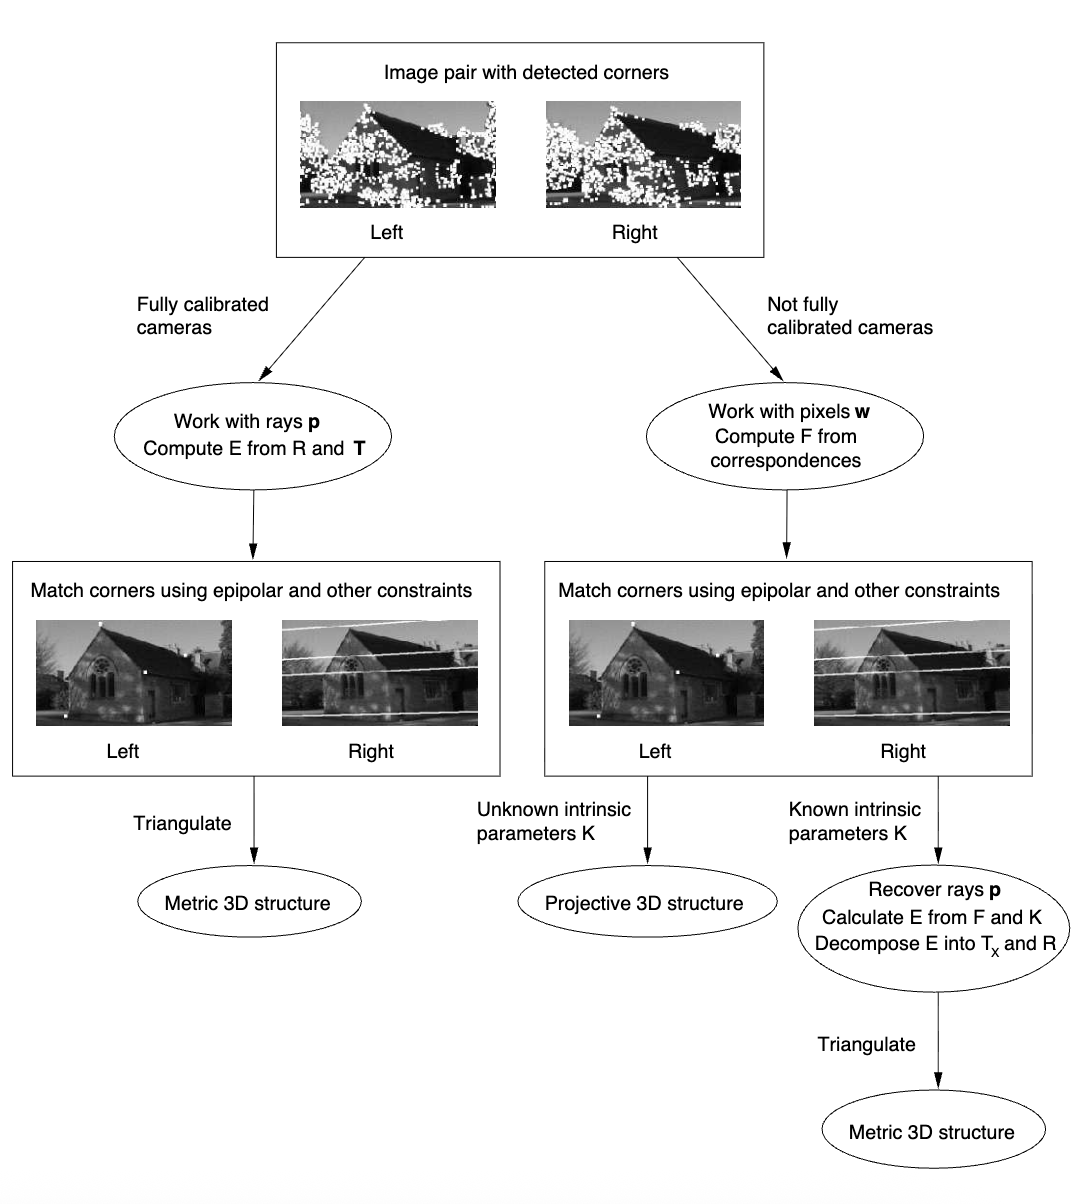
\includegraphics[width=0.7\textwidth]{figures/4F12/stereo.png}
\end{center}

\textbf{Affine stereo:} When the depth of the scene is small compared to the distance from the camera, the affine camera is appropriate:
$$
\begin{bmatrix}u \\ v \\ u' \\ v' \end{bmatrix} = \begin{bmatrix}p_{11} & p_{12} & p_{13} & p_{14} \\ p_{21} & p_{22} & p_{23} & p_{24} \\ p_{11}' & p_{12}' & p_{13}' & p_{14}' \\ p_{21}' & p_{22}' & p_{23}' & p_{24}' \end{bmatrix} \begin{bmatrix}X \\ Y \\ Z \\ 1\end{bmatrix}
$$

Assuming the left camera is aligned with the world coordinate, the left projection matrix is $\begin{bmatrix}
    p_{11} & 0 & 0 & p_{14} \\
    0 & p_{22} & 0 & p_{24} \\
\end{bmatrix}$. Substitution yields the epipolar constraint: $$\mathbf{w}' = \mathbf{a} + Z \mathbf{b}$$ $\mathbf{b}$ is independent of $\mathbf{w}$ so all epipolar lines are parallel under affine stereo.

\textbf{Affine fundamental matrix:} The affine fundamental matrix is 
$$
\mathrm{F}_A = \begin{bmatrix}
    0 & 0 & a \\
    0 & 0 & b \\
    c & d & 1
\end{bmatrix} \quad \text{such that} \quad
\tilde{\mathbf{w}}'^\top \mathrm{F}_A \tilde{\mathbf{w}} = 0
$$

\newpage
\section{Deep Learning for Computer Vision}
\textit{Note: The following notes may not be comprehensive and are intended to provide a high-level overview of the key concepts.}

\textbf{Perceptron:} $y(\mathbf{x}) = f(\mathbf{w}^\top \mathbf{x} + b)$, where $f$ is the activation function (e.g. $\tanh$).

\textbf{Cross-entropy loss:} $L = -\sum_i y_i \log \hat{y}_i$.

\textbf{Batching:} Use a subset of data to compute gradients and update weights and biases. It is known as \textit{stochastic gradient descent} when the subsets are chosen at random.

\textbf{Division of data:}
\begin{enumerate}
    \item Training -- fitting the model
    \item Validation -- determining the hyperparameters
    \item Test -- held out for evaluation
\end{enumerate}

\textbf{Rectified Linear Unit (ReLU):} $f(x) = \max(0, x)$, used to solve the vanishing gradient problem of sigmoid and $\tanh$.

\textbf{Convolution:} Computing the dot product between a kernel and a local region of input (e.g. image patch).

\textbf{Subsampling:} Reducing the dimensionality of the convolution layer output by taking the maximum (max pooling) or average (average pooling) of a local region.

\textbf{Convolutional Neural Networks (CNNs):} 
\begin{center}
    \includegraphics[width=0.5\textwidth]{figures/4F12/cnn.png}
\end{center}

\textbf{Network in Network (NiN):} Replace the fully connected layers with $1 \times 1$ convolution, which can be seen as a MLP applied across filter channels.

\textbf{Semantic segmentation:} Assign a class label to each pixel in the image. Replace the final classifier with an an interpolation layer.

\textbf{Autoencoding:} Encoding the input into a latent space and decoding it back to the original input.

A \textit{variational autoencoder} encodes the input into two vectors $\mu$ and $\sigma$ and the system samples from $\mathcal{N}(\mu, \sigma)$ as the latent space input to the decoder. The loss function is the \textit{evidence lower bound} (ELBO):
$$
\mathcal{L} = \mathbb{E}_{q(z|x)}[\log p(x|z)] - D_{KL}(q(z|x) || p(z))
$$
where the first term is the reconstruction loss (trains the generative decoder distribution to transform the latent vector back to input) and the second term is the regularisation loss (trains the encoder distribution $q(z|x)$ to be close to $p(z) = \mathcal{N}(0, I)$).

\textbf{Transposed convolution:} Increase the output dimension by scaling a kernel by an input pixel value and add it to a patch of the output image.
\begin{center}
    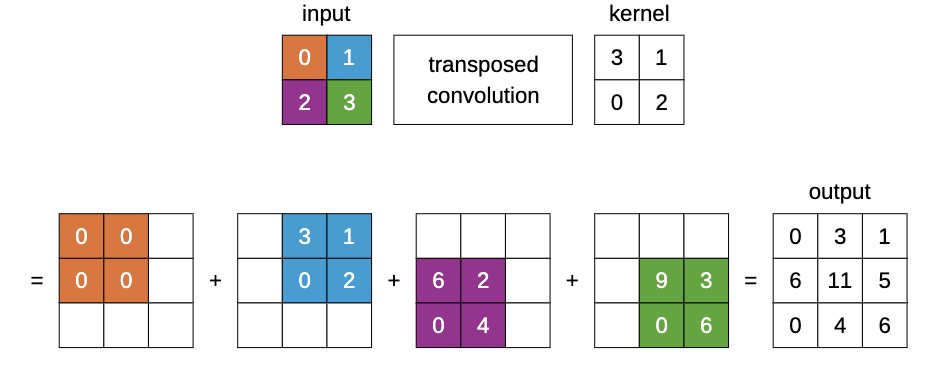
\includegraphics[width=0.6\textwidth]{figures/4F12/transposed_convolution.png}
\end{center}

\textbf{Instance segmentation (object detection):} Assign multiple members of a class different labels.

\textbf{You Only Look Once (YOLO):} A network that divides the image into a grid of cells, and for each cell predict a set of bounding boxes and a class label for each box.

\textbf{Feature embedding:} Latent space representation such that similar inputs are close together and dissimilar inputs are larger. The $\textit{triplet loss}$ can be used for training:
$$
\mathcal{L} = \sum_{i=1}^N \max(0, \|\mathbf{z}_a^i - \mathbf{z}_p^i\|_2^2 - \|\mathbf{z}_a^i - \mathbf{z}_n^i\|_2^2 + \alpha)
$$
where the triplets are anchor point $a$, positive point $p$, and negative point $n$.

\textbf{Positional encoding:} Represent a function by a combination of sine and cosine functions of different frequencies.

\textbf{Sampling from transformers:} A couple of options:
\begin{itemize}
    \item Sample from the output distribution, which can be adjusted by a temperature.
    \item Top-k sampling: Sample from the top $k$ most probable tokens.
    \item Beam search: Keep track of the top $k$ most probable sequences at each step and expand them in the next step. Select the most probable sequence at the end.
\end{itemize}

\end{document}
